% 天文学常识
% 天文学|天球|四季|太阳系|行星|恒星

\subsection{太阳系模型}

\begin{figure}[ht]
\centering
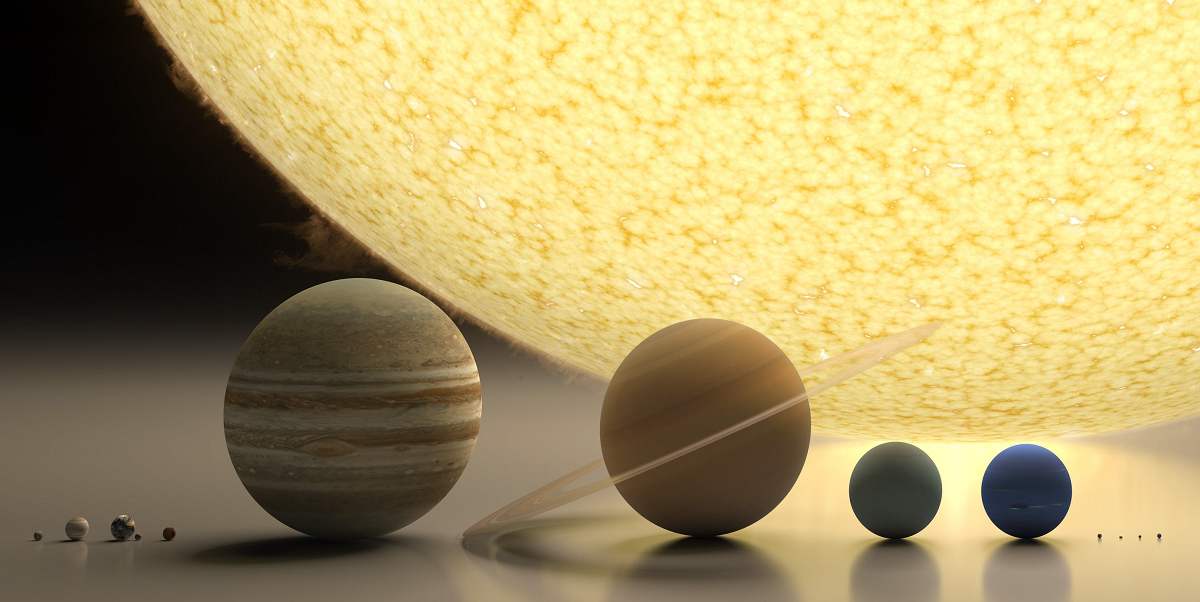
\includegraphics[width=14cm]{./figures/Astro_1.png}
\caption{真实比例下太阳与行星的大小(来自 pinterest.com), 行星从左到右依次为水星, 金星, 地球(及月亮), 火星, 木星, 土星, 天王星, 海王星, 其他小行星} \label{Astro_fig1}
\end{figure}

恒星和行星一个显著的区别就是恒星很大, 而且会发光. 太阳是太阳系中唯一一个恒星, 其他天体都不发光, 而是反射太阳的光.

关于太阳系模型一个误区是行星的尺寸和距离, 几乎所有(实物的)太阳系模型的比例都是完全错误的, 原因是如果按照真实比例制作模型, 要么就是行星小得看不到, 要么就是模型大得不切实际. 我们这里来构建一个符合比例的太阳系模型, 即用乒乓球来代表太阳, 再按比例计算其他长度和距离, 结果见\autoref{Astro_tab1}.

\begin{table}[ht]
\centering
\caption{太阳系的一些数据}\label{Astro_tab1}
\begin{tabular}{|c|c|c|}
\hline
 & 真实长度 & 模型长度 \\
\hline
太阳半径 & $6.96\times 10^5 \Si{km}$ & $20.0 \Si{mm}$\\
\hline
地球半径 &  $6.37\times 10^3 \Si{km}$ & $0.183 \Si{mm}$\\
\hline
地球到太阳  &  $1.46 \times 10^8 \Si{km}$ & $4.20 \Si{m}$\\
\hline
月球半径 & $1.74 \times 10^3 \Si{km}$ & $0.0500 \Si{mm}$\\
\hline
月球到地球 & $3.84 \times 10^5 \Si{km}$ &  $1.10 \Si{cm}$\\
\hline
木星半径 & $7.15 \times 10^4 \Si{km}$ & $2.05 \Si{mm}$\\
\hline
木星到太阳 & $7.79 \times 10^8 \Si{km}$ & $22.4 \Si{m}$\\
\hline
海王星到太阳 & $4.50 \times 10^9 \Si{km}$ & $129 \Si{m}$\\
\hline
最近的恒星到太阳 & $3.99 \times 10^{13} \Si{km}$ &  $1.15 \times 10^3 \Si{km}$\\
\hline
\end{tabular}
\end{table}
注意最后一栏中, 即使按照模型的比例, 最近的恒星离我们也有 1000 多公里, 可见宇宙是相当空旷的.

\subsection{星空}

\begin{figure}[ht]
\centering
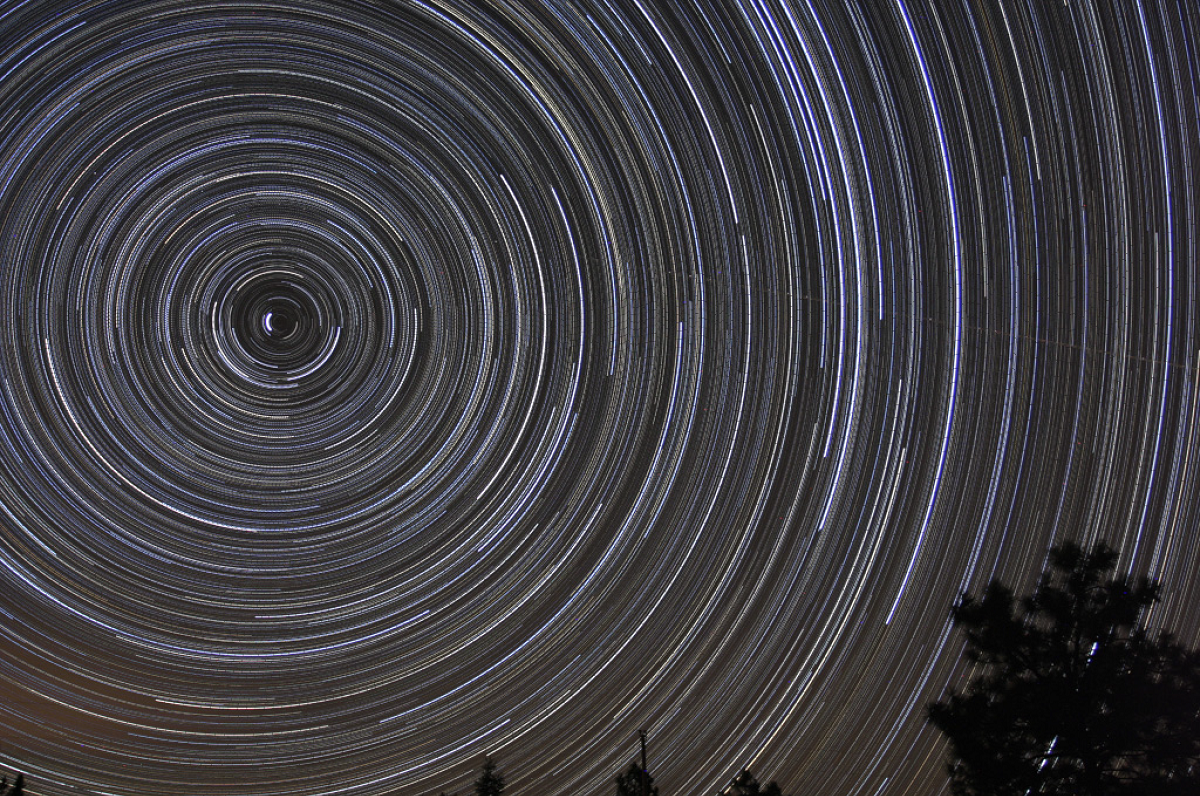
\includegraphics[width=14cm]{./figures/Astro_2.png}
\caption{星星的轨迹(来自 burro.case.edu), 注意如果测量图中每条弧线的张角就可以计算曝光的时间} \label{Astro_fig2}
\end{figure}

除了太阳系中的天体, 肉眼或望远镜能看到的其他星星都属于恒星(注意有一些亮点是星云, 即星际尘埃而不是单个恒星), 离太阳最近的恒星叫做 Alpha Centauri (4.22 光年). 由于这些恒星的距离太远, 即使用天文望远镜也看不到它们的行星. 恒星在空中的相对位置是几乎不变的(即使太阳系以惊人的速度绕星系中心旋转, 但转一圈仍需要 2.3 亿年, 所以与其他恒星的相对位置基本保持不变).

那我们看到的星空是如何变化的呢? 由于地球每 24 小时由西向东自转一圈, 所以我们在地球上看到的星空由东向西围绕地球旋转. 长时间曝光的照片可以很好地展示星星的轨迹(\autoref{Astro_fig2}). 如果站在北极点, 那么星空的旋转中心会在正上方, 如果站在赤道, 旋转中心会在地平线上, 且南北各有一个. 如果站在南极点, 则旋转中心同样在正上方但旋转方向却与北极的相反.

一个常见的问题是为什么白天看不到星星和月亮. 这是因为白天阳光照亮了大气中的尘埃和云, 相比之下星星的亮度太暗了所以肉眼不容易看到. 许多时候月亮也会在白天出现, 只是因为阳光太亮不容易注意到.

\subsection{季节与昼夜}

\begin{figure}[ht]
\centering
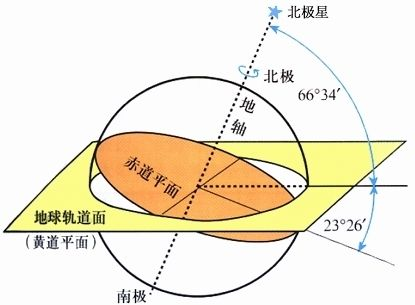
\includegraphics[width=9cm]{./figures/Astro_4.png}
\caption{黄赤交角示意图} \label{Astro_fig4}
\end{figure}

如\autoref{Astro_fig4}, 地球绕太阳公转轨道所在的平面叫\textbf{黄道平面}, 而地轴与黄道平面有大约 $23.5^\circ$ 的倾角, 所以当地球运动到太阳的一侧时, 太阳直射到\textbf{北回归线}(北纬 $23.5^\circ$ 的纬线), 这一天就叫做\textbf{夏至}, 当地球绕太阳旋转 $90^\circ$ 后, 太阳直射到赤道上, 这一天就叫做\textbf{秋分}, 而地球再公转 $90^\circ$ 到另一侧时, 太阳直射到南回归线, 这一天就是\textbf{冬至}, 再公转 $90^\circ$, 阳光再次直射到赤道上, 这一天就是\textbf{春分}. 注意这是对北半球而言, 南半球相反.因此季节的变化本质上是太阳直射点的变化,与地球与太阳的距离关系不大,事实上在北半球的冬季地球到太阳的距离要小于夏季的距离. 

回想第一节的太阳系模型, 由于地球到太阳的距离远大于二者的半径, 所以可以近似认为太阳照到地球的光都是平行的, %(图未完成)
这样, 任何时刻只有半个地球被照亮, 这半个地球就是白天, 而另外半个是晚上. 由于地轴的倾斜, 北半球某条纬线以上的地区在夏天会被全部被照亮, 这样无论地球自转多少, 这些地区都是白天, 这就形成了\textbf{极昼}. 与此同时, 南半球某条纬线以上的地区全部没有阳光, 就形成了\textbf{极夜}. 同理, 在冬天(也就是南半球的夏天)南极附近会出现极昼而北极附近出现极夜. 另外在赤道, \textbf{昼长}(白天的长度)和\textbf{夜长}(夜晚的长度)一年四季都相等.

\subsection{天球坐标系}

下面我们来更具体地描述星空.由于天体离我们足够遥远,来自天体的光线已近似于平行光,这时候我们已经失去了确定远近的能力(当然事实上我们有其他的办法确定天体的视向距离),而仅仅知道天体的方位,所有的天体都彷佛分布在一个球面上.假定围绕着我们有一个大圆球,它的半径比我们所能看到的最远的天体的距离还要大得多,这个假想的球体称为\textbf{天球}.观测者总是处于天球的中心,这是因为观测者的任意位移(包括地球的公转)都比天球半径小得多,可以忽略不计.天体和观测者眼睛连成的直线与天球面的交点,也就是天体在天球面上的投影,称为天体的\textbf{视位置}.

为了定量地表述天体在天球上的位置,我们需要建立球坐标系(正如我们描述地球上某个地点需要使用经度和纬度一样),最常用的两个天球坐标系是\textbf{地平坐标系}和\textbf{赤道坐标系}.

\begin{figure}[ht]
\centering
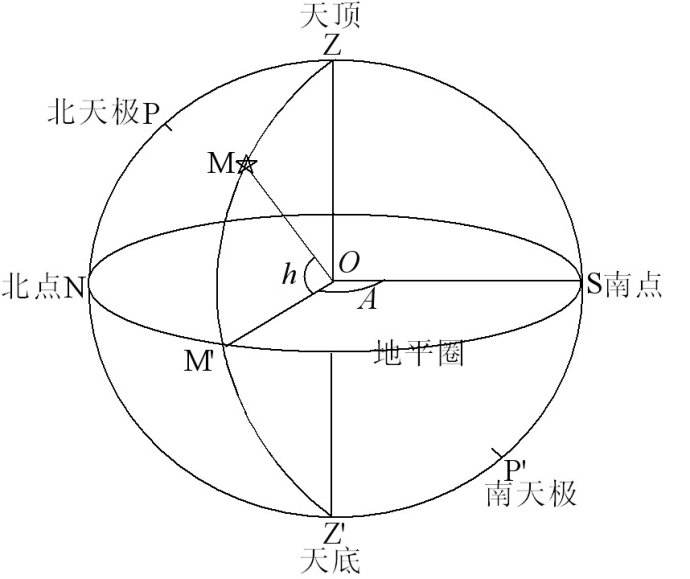
\includegraphics[width=9cm]{./figures/Astro_5.png}
\caption{地平坐标系} \label{Astro_fig5}
\end{figure}

地平坐标系(\autoref{Astro_fig5})是以观测者的位置为基础建立的,是最自然的坐标系.观测者立直站在地平面上,通过观测者和天球心的直线在天球上有两个交点,头顶 $Z$ 称为\textbf{天顶},脚下 $Z'$ 称为\textbf{天底},与该直线垂直的平面叫做天球地平面,与天球相交的大圆称为\textbf{地平圈},也叫\textbf{真地平}.过天顶和北天极(地轴北极与天球的交点)的大圆称为\textbf{天子午圈},天子午圈和真地平相交于 $N$ 和 $S$ 点, $N$ 点靠近北天极,称为\textbf{南点},其实和我们通常所说的东南西北的概念是一致的.天球上天体的坐标用\textbf{地平经度} $A$ 和\textbf{地平纬度} $h$ 来描述,具体的度量方法已在图上标注,有时候也称\textbf{方位角}和\textbf{高度}.对于北天极,很容易证明它的地平高度恰好等于该地的纬度.

\begin{figure}[ht]
\centering
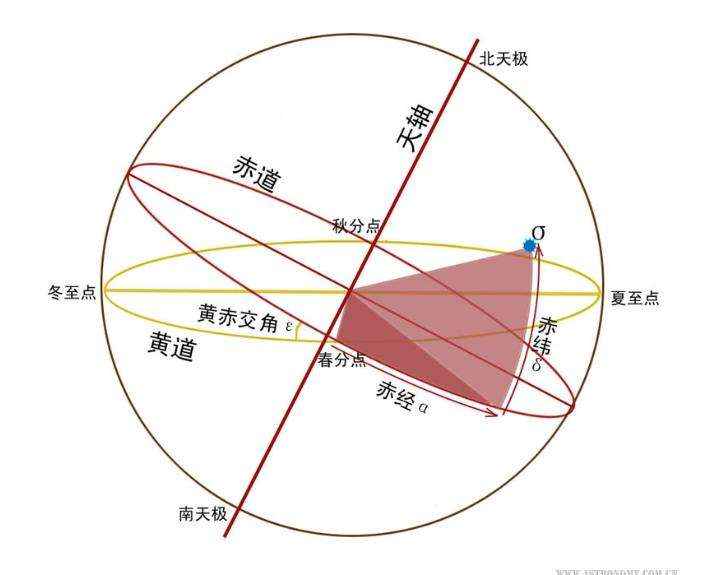
\includegraphics[width=12cm]{./figures/Astro_6.png}
\caption{赤道坐标系} \label{Astro_fig6}
\end{figure}

尽管地平坐标系在日常观星时很常用,但是同一个天体的坐标会随着观测地点的不同而不同,在实际的天文观测中,最常使用的坐标系称为\textbf{赤道坐标系}(\autoref{Astro_fig6}).我们将地球的赤道面无限延展,与天球相交的大圆称为\textbf{天赤道}.地球公转轨道面延伸与天球相交的大圆称为\textbf{黄道},黄道事实上是太阳相对于星空背景运动的轨迹,一年运动一圈,人们也常常把这种运动叫做太阳的周年视运动.天赤道与黄道有两个交点,分别称为\textbf{春分点}和\textbf{秋分点},其中春分点是太阳视运动沿着黄道从天赤道以南穿过天赤道以北的交点,秋分点则相反.赤道坐标系中天体的坐标用\textbf{赤经}和\textbf{赤纬}来度量,具体的度量方法在图上标出.天体的赤经和赤纬是不会随观测地点、观测时间的改变而改变的.

\subsection{天体的周日视运动}

\begin{figure}[ht]
\centering
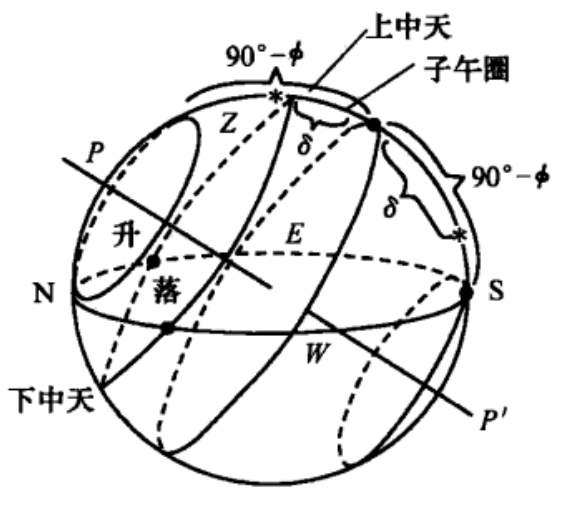
\includegraphics[width=9cm]{./figures/Astro_7.png}
\caption{周日视运动} \label{Astro_fig7}
\end{figure}

在地平坐标系中,人们站在地球上不觉得地球在自转,只看到天球带动所有天体绕着天轴在反方向旋转,只有北天极和南天极两点不动,这种运动称为天球的\textbf{周日视运动}.恒星因为周日视运动在天球上画出了一系列平行的圈(\autoref{Astro_fig7}),我们称天体高度角达到最大的时候为\textbf{上中天},相反为下中天,事实上就是天体通过天子午圈的时候上/下中天.容易发现,有一些天体永远不会落下,有些天体也永远不会升起,这是由天体的赤纬和观测地点的纬度共同决定的.
